\begin{abstract}
Electrophysiological foundation models must accommodate changes in sensor hardware, including wearable optically pumped magnetometers (OPMs). We test how one pretrained model, BrainOmni, behaves when the recording hardware changes, using only input interventions and no weight updates. Relabelling radial OPM magnetometers as gradiometers raises zero-shot waveform reconstruction from $0.2501$ to $0.3819$ Pearson correlation in all 21 participants of a single-axis cohort, and moves the same way in a single-participant SQUID diagnostic. The effect is configuration-dependent: on a triaxial cohort, the monolithic tag contrast is $\FxRawTagMonolithicMean$ ($p=\FxRawTagMonolithicP$). A factorial crossing tag, filtering and partition shows that axis grouping beats an exactly size-matched random partition averaged over ten seeds under both tags. With soft homogeneous field correction (Soft-HFC), the advantage is $\FxSofthfcMagGroupingMean$ under MAG and $\FxSofthfcGradGroupingMean$ under GRAD, each in $\FxSofthfcMagGroupingCount$ participants. The paired interaction is $\FxSofthfcInteractionMean$: the grouping advantage is smaller under the GRAD tag. Reconstruction gains do not establish decoding gains. On tactile Braille classification, a classical decoder over six log band powers and four temporal window means per channel clears chance under Soft-HFC while the pretrained probe does not. At ten participants, the decoding results remain inconclusive. These findings motivate testing continuous sensor parameterization and axis-conditioned queries, with reconstruction and decoding evaluated separately against competitive baselines.
\end{abstract}

\section{Introduction}
Learning across heterogeneous biosignal recordings requires representations that accommodate differences in channel configuration and acquisition format. BIOT addresses mismatched channels, variable recording lengths and missing values by tokenizing channels separately and combining the tokens with channel and temporal embeddings \citep{yang2023biot}. LaBraM learns reusable EEG representations through channel patches and masked neural-code prediction \citep{jiang2024labram}. BrainOmni extends representation learning to joint EEG and MEG data through sensor-conditioned tokenization and masked-token modeling \citep{xiao2025brainomni}. These approaches motivate examining how a frozen model responds to changes in sensor hardware and metadata.

OPM-MEG provides a concrete setting for this question. \citet{boto2017opm} demonstrated near-scalp OPM measurements of evoked and induced somatosensory activity without cryogenic cooling. \citet{boto2018wearable} subsequently demonstrated a wearable MEG system that records brain activity during natural head movement. These developments allow flexible sensor placement, while triaxial systems measure three orthogonal field components \citep{rea2022triaxial}. The resulting changes in sensor geometry and channel organization motivate testing the sensor-conditioning interface of a model transferred to OPM recordings.

OPM-MEG is therefore a stress test for the sensor-conditioning interface, which is where hardware enters the computation. We hold the weights fixed and intervene only on what the model is told about its sensors: the categorical tag, the position and orientation vectors, and the grouping of channels passed through spatial attention. The question is not whether the model can be fine-tuned onto OPM data, but which inputs its representation is sensitive to, and whether those changes survive as decoding gains.

Our contributions are: (i) a paired, per-participant quantification of sensor-type and geometry sensitivity on two public OPM cohorts with a SQUID diagnostic; (ii) a preprocessing-matched comparison of axis grouping against a random control with matching group sizes and pass count; and (iii) improved reconstruction without a detectable improvement in linear decoding against a competitive classical baseline.

\section{Data and Evaluation}

\subsection{Datasets}

\textbf{Single-axis OPM.} FACE-DEC, OpenNeuro ds005107 \citep{xu2024face}. We use 21 participants and the 50 channels matched by rounded position and orientation metadata. The documentation states that coordinates were approximated from an Elekta layout for display and are not measured OPM positions \citep{facedecdocs}, so a shared channel set is not evidence of anatomical alignment and spatial perturbations test the model's response to supplied metadata.

\noindent \textbf{Triaxial OPM.} The 10 adult participants of Zenodo record 11126593 \citep{rier2024dataset}, 84 cached trials each, 155--176 retained channels, geometry in head coordinates. The task contrasts index-finger and little-finger stimulation; results apply to this adult subset, not the full developmental cohort.

\noindent \textbf{SQUID diagnostic.} Participant sub-01, run-01 of OpenNeuro ds000117 \citep{wakeman2015}, with 102 magnetometers and 204 planar gradiometers. This is a single-participant diagnostic used only to test whether the sensor-type effect is OPM-specific.

\subsection{Model, Endpoint and Interventions}
We evaluate the pretrained BrainOmni tiny configuration. Its tokenizer combines a temporal convolutional encoder with spatial cross-attention between 16 learned queries and per-channel embeddings of position, unit orientation and discrete sensor type, followed by residual vector quantization. The sequence backbone is bidirectional and trained by masked-token prediction over codebook entries, not autoregressively. Reconstruction uses the tokenizer encoder, quantizer and decoder with weights frozen. Here zero-shot means evaluation without OPM-specific weight updates. The complete input is supplied to the tokenizer: this is unmasked reconstruction, not prediction of held-out samples or missing channels.

The primary endpoint is Pearson correlation (PCC) between the reconstructed and the normalized input waveform window. Higher PCC means closer agreement with the observed input, which still contains artifact, not better source localization or denoising. The triaxial factorial averages per-trial PCC within participant.

Interventions on the single-axis array reassign the sensor tag from magnetometer (\texttt{MAG=1}) to gradiometer (\texttt{GRAD=2}), zero the orientation vectors, reverse them, or jointly permute position and orientation across channels, in every case leaving the waveforms untouched. All single-axis conditions share channel selection and a soft variant of homogeneous field correction \citep{tierney2021hfc}: Soft-HFC, $P = I - \alpha Q_R Q_R^{\top}$ with $\alpha = 0.25$, where $Q_R$ is an orthonormal basis for the sensor-orientation subspace. Soft-HFC attenuates any component projecting onto that subspace, including neural signal, so its effect is separated from tokenization throughout; Supplementary Section~\ref{sec:soft-hfc} derives it.

For triaxial arrays the monolithic tokenizer passes all retained channels through one spatial bank. Axis partitioning passes the $X$, $Y$ and $Z$ groups separately through the same pretrained tokenizer and reassembles the reconstructions, giving three 16-query passes instead of one. The random control uses ten seeds and exactly matches each participant's $Z$, $X$ and $Y$ group sizes. We average seeds within participant before inference. Here and throughout, \emph{raw} denotes cached, preprocessed inputs without additional Soft-HFC, not unprocessed recordings. The supplied triaxial caching script applies 50 and 100 Hz notch filters, a 1--45 Hz bandpass, epochs from $-0.2$ to $1.8$ seconds with prestimulus baseline correction, and resamples to 256 Hz. The factorial operates on 512-sample cached trials. These settings describe the supplied implementation; raw-data replay has not been verified. Crossing MAG/GRAD tags, raw/Soft-HFC inputs and monolithic/random/axis partitions gives a $2\times2\times3$ factorial; contrasts hold filtering constant.

\subsection{Statistics}
All comparisons are paired within participant. We report the mean paired difference with a percentile bootstrap confidence interval over participants (20{,}000 resamples), the number of participants in which the difference has the stated sign, and an exact two-sided sign-flip permutation $p$-value enumerating all $2^{n}$ assignments. With $n=10$ the smallest attainable $p$ is $2/2^{10} \approx 0.002$, so triaxial $p$-values at that value indicate perfect consistency rather than a precisely estimated tail. These intervals condition on the saved predictions, fixed cross-validation splits and evaluated partition seeds; they do not include variation from retraining, alternative splits or new recording sessions. Tests are exploratory and unadjusted for multiple comparisons. The supplement gives participant values, seed sensitivity and the complete decoding comparisons.


\begin{figure}[t]
\centering
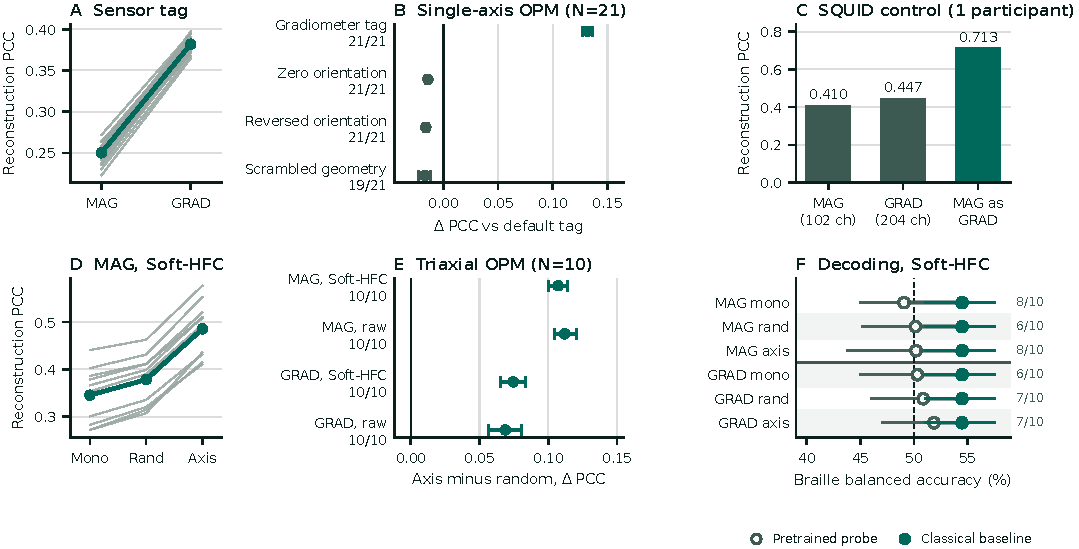
\includegraphics[width=\textwidth]{figures/transfer_overview.pdf}
\caption{Paired per-participant reconstruction and decoding results. \textbf{A}, \textbf{D}: paired trajectories, one grey line per participant, cohort mean in colour; \textbf{D} traces MAG-tag monolithic, ten-seed random and axis partitions under Soft-HFC. \textbf{B}, \textbf{E}: mean paired differences with participant bootstrap 95\% intervals; the count under each label gives participants moving in the stated direction. \textbf{B} is against the default magnetometer tag; \textbf{E} gives axis-minus-random contrasts for both tags and filters. \textbf{C}: single-participant SQUID diagnostic. \textbf{F}: full-array Braille decoding under Soft-HFC for both tags, probe (open) against classical baseline (filled), dashed line at chance; the right column counts participants where classical exceeds probe. Random-partition decoding uses seed 42 with axis-matched group sizes. The classical arm is invariant to tag and partition.}
\label{fig:overview}
\end{figure}

\section{Results}

\subsection{A Discrete Label Dominates Reconstruction}
Table~\ref{tab:single} and Figure~\ref{fig:overview}A,B give the single-axis results; per-participant values are in supplement Tables S1 and S2. Relabelling the array from magnetometer to gradiometer, with waveforms, positions and orientations unchanged, raises reconstruction from $0.2501$ to $0.3819$, a paired difference of $+0.1318$ (95\% CI $[+0.1275, +0.1360]$), a relative increase of 52.7\%. The effect holds in 21 of 21 participants with no overlap between the two distributions, exact $p < 10^{-5}$. The SQUID diagnostic moves in the same direction and further: magnetometer-only reconstruction rises from $0.4105$ to $0.7130$ when those 102 native SQUID magnetometers are assigned the gradiometer category, a 73.7\% relative increase, on hardware the model was pretrained on.

Because the intervention changes one categorical token and nothing numerical, the result isolates a property of the learned embedding rather than of the recording. It is consistent with the gradiometer subspace having absorbed most of the MEG pretraining signal. A simpler account is that the two embeddings carry learned gain and unit priors and that OPM amplitude statistics sit nearer the gradiometer prior. These predict differently under a continuous parameterization, and this design cannot separate them. The triaxial factorial below limits either account: a tag advantage on one cohort does not establish a general preference for the gradiometer category.

The geometry perturbations move in the opposite direction and are small: zeroing orientations costs $-0.0142$ ($\SaZeroOrientationCount$ participants declined), reversing them $-0.0161$ ($\SaFlipOrientationCount$ declined), and scrambling position and orientation jointly $-0.0171$ ($\SaScrambleChannelsCount$ declined). The tokenizer does read the directional vectors, but on this cohort the discrete tag is seven to nine times more consequential than the continuous geometry, depending on which perturbation is the comparator. Scrambling approximate coordinates may scramble little, so this bounds the tag against the metadata quality of this cohort rather than against geometry as such.

\begin{table}[tb]
\centering
\small
\setlength{\tabcolsep}{4pt}
\begin{tabular}{lrr}
\toprule
Condition & PCC [95\% CI] & $\Delta$ (consist.) \\
\midrule
Default (\texttt{MAG=1}) & .2501 [.2450, .2549] & baseline \\
Gradiometer tag & .3819 [.3779, .3859] & $+.1318$ (21/21) \\
Zero orientation & .2359 [.2295, .2421] & $-.0142$ (\SaZeroOrientationCount) \\
Reversed orient. & .2340 [.2274, .2402] & $-.0161$ (\SaFlipOrientationCount) \\
Scrambled geometry & .2330 [.2307, .2354] & $-.0171$ (\SaScrambleChannelsCount) \\
\bottomrule
\end{tabular}
\caption{Waveform reconstruction on FACE-DEC (21 participants, 50 shared channels, Soft-HFC $\alpha = 0.25$). $\Delta$ is the mean paired difference against the default tag; consistency counts participants moving in that direction. Coordinates are approximate, which limits anatomical interpretation of the geometry rows.}
\label{tab:single}
\end{table}

\subsection{Tag and Axis Grouping Interact}
\begin{table}[tb]
\centering\small
\setlength{\tabcolsep}{4pt}
\begin{tabular}{llrr}
\toprule
Partition & HFC & MAG PCC & GRAD PCC \\
\midrule
Monolithic & no & \FxRawMagMonolithicMean & \FxRawGradMonolithicMean \\
Random & no & \FxRawMagRandomMean & \FxRawGradRandomMean \\
Axis & no & \FxRawMagAxisPartitionedMean & \FxRawGradAxisPartitionedMean \\
Monolithic & Soft & \FxSofthfcMagMonolithicMean & \FxSofthfcGradMonolithicMean \\
Random & Soft & \FxSofthfcMagRandomMean & \FxSofthfcGradRandomMean \\
Axis & Soft & \FxSofthfcMagAxisPartitionedMean & \FxSofthfcGradAxisPartitionedMean \\
\bottomrule
\end{tabular}
\caption{Full-array triaxial factorial, 10 adults, 84 trials each. Trial-weighted participant PCC; random partitions average ten seeds with group sizes matched to each participant's axes. Supplement Tables S3--S6 give intervals, paired contrasts, participant values and seed sensitivity.}
\label{tab:tri}
\end{table}
Table~\ref{tab:tri} crosses tag, filtering and partition. Against the ten-seed random mean, axis partitioning gains $\FxSofthfcMagGroupingMean$ ($\FxSofthfcMagGroupingCI$) under MAG with Soft-HFC and $\FxRawMagGroupingMean$ ($\FxRawMagGroupingCI$) without it. Under GRAD the gains remain $\FxSofthfcGradGroupingMean$ ($\FxSofthfcGradGroupingCI$) and $\FxRawGradGroupingMean$ ($\FxRawGradGroupingCI$). All four contrasts are positive in $\FxSofthfcMagGroupingCount$ participants ($p=\FxSofthfcMagGroupingP$). Under Soft-HFC/MAG, the seed-specific cohort gains range from $\FxSofthfcMagMinimum$ to $\FxSofthfcMagMaximum$ (SD $\FxSofthfcMagSd$), so the result persists across partitions.

The tag effect depends on partition. GRAD minus MAG is $\FxRawTagMonolithicMean$ ($\FxRawTagMonolithicCI$, $\FxRawTagMonolithicCount$, $p=\FxRawTagMonolithicP$) on raw monolithic inputs, and $\FxSofthfcTagMonolithicMean$ ($p=\FxSofthfcTagMonolithicP$) under Soft-HFC. These estimates give no evidence of the large FACE-DEC advantage, without establishing equivalence. Under Soft-HFC, remapping helps the random partition by $\FxSofthfcTagRandomMean$ ($p=\FxSofthfcTagRandomP$); on raw axis partitions it changes PCC by $\FxRawTagAxisPartitionedMean$ ($p=\FxRawTagAxisPartitionedP$). The paired change in axis-minus-random gain from MAG to GRAD is $\FxSofthfcInteractionMean$ ($\FxSofthfcInteractionCI$) under Soft-HFC and $\FxRawInteractionMean$ ($\FxRawInteractionCI$) raw, both $p=\FxRawInteractionP$. Grouping survives, but its advantage and the tag effect partly overlap.

The monolithic-to-random contrasts are tag-conditional too. Under Soft-HFC, random minus monolithic is $\FxSofthfcMagMonoToRandomMean$ under MAG and $\FxSofthfcGradMonoToRandomMean$ under GRAD. These account for $\FxSofthfcMagMonoToRandomPercent\%$ and $\FxSofthfcGradMonoToRandomPercent\%$ of the respective axis-over-monolithic gains. These are descriptive partition components: random partitioning changes attention composition as well as query budget. A matched-query monolithic control remains missing, so a capacity contribution cannot be isolated.

\subsection{No Detectable Improvement in Linear Decoding}
The full-array factorial evaluates tactile Braille decoding across both tags, both filtering regimes and all three partitions. Random-partition decoding uses seed 42 with axis-matched group sizes. Figure~\ref{fig:overview}F shows the six Soft-HFC configurations; supplement Table S7 gives all twelve configurations and the random-initialization control. The pretrained linear probe has means from \FxProbeMinimum\% to \FxProbeMaximum\%, with every participant-bootstrap interval including chance. Paired axis-minus-monolithic and axis-minus-random decoding contrasts also have intervals spanning zero in every tag/filter combination (supplement Table S8).

The classical baseline uses six log band powers spanning 1--96\,Hz plus four temporal window means per channel, classified by $L_2$-regularized logistic regression. It reaches \FxClassicalSofthfcMean\% $\FxClassicalSofthfcCI$ under Soft-HFC and \FxClassicalRawMean\% $\FxClassicalRawCI$ without additional Soft-HFC. Its features depend on filtering but not on the sensor tag or tokenizer partition, so the six rows within each filtering regime share one classical measurement. Only the Soft-HFC interval excludes chance. The classical cohort mean exceeds the pretrained probe in all twelve configurations, although this ordering alone does not establish a significant paired advantage.

We observe improved reconstruction without a detectable improvement in linear decoding. With ten participants, these results remain inconclusive and do not establish equivalence. A larger cohort is needed to distinguish limitations of the representation from task difficulty.

\section{Discussion and Limitations}
Two design hypotheses follow. First, continuous sensor metadata merits testing against the categorical interface. A continuous parameterization, such as stand-off distance and baseline length, would let a new sensor occupy its own place instead of borrowing a category, and is testable against the categorical baseline. The 52.7\% FACE-DEC gain is configuration-dependent; the triaxial monolithic estimates do not support its generalization, and the cohorts differ in more than axis count.

Second, axis-conditioned spatial queries merit testing in multi-axis arrays. Grouping retains an advantage under both tags, although its magnitude depends on the tag. The tested partition retains every channel but prevents joint spatial attention across axis groups. It uses three tokenizer passes over smaller channel sets and increases the aggregate query count from 16 to 48; runtime and FLOPs were not benchmarked. Axis-conditioned queries inside one bank would provide a further test of grouping while permitting cross-axis information exchange. Their reconstruction performance and computational cost remain untested.

The limits are real. We evaluate one model on two small OPM cohorts with a single-participant SQUID diagnostic, so no harmonized cross-hardware estimate follows. FACE-DEC coordinates are approximate. Ten random seeds and the crossed tag design strengthen the grouping result, but the monolithic tokenizer still lacks a matched token budget. The algebraic decomposition cannot identify capacity and grouping mechanisms separately. Every positive result uses correlation to the processed input, so a model can gain by matching artifact structure. An artifact-robust endpoint is needed to test whether the reconstruction gains reflect neural signal. Results are based on cached inputs and saved model outputs; raw-data replay remains untested.

\section{Conclusion}
Sensor metadata and channel grouping shape zero-shot reconstruction in configuration-dependent ways. The large single-axis tag effect is absent from the triaxial monolithic point estimates, while axis grouping retains an advantage under both tags. Their interaction shows that the grouping advantage depends on the sensor tag in this factorial. These reconstruction improvements do not establish better decoding; continuous sensor parameterization and axis-conditioned queries remain hypotheses to test against competitive baselines.

\section*{Data and Code Availability}
The datasets are identified in Supplementary Section~\ref{sec:datasets}. The analysis repository is \url{https://github.com/samerzumot/opm-bridge}. The accompanying implementation includes the factorial runner, saved aggregate and per-trial results, and scripts that regenerate the reported tables and figures. The pretrained model is distributed separately by OpenTSLab as BrainOmni. Verification for this version recalculated statistics from the saved records and checked the supplied code; it did not replay raw recordings or verify the original checkpoint execution environment.

\section*{Ethics and Data Use}
This is a secondary analysis of three publicly available datasets, identified by accession and DOI in Supplementary Section~\ref{sec:datasets}. No new recordings were made and no participants were recruited for this work. Ethical approval and participant consent for the original acquisitions rest with the studies that produced them. We used the de-identified data as distributed, made no attempt at re-identification, and redistribute no participant-level recordings: the accompanying repository contains derived aggregate and per-trial statistics only. Terms of reuse for the underlying recordings are those stated by each source repository.

\section*{Funding}
This work received no external funding.

\section*{Competing Interests}
S.Z. undertakes independent commercial work in neurotechnology related to the application area of this study. This had no role in the design of the analyses, the interpretation of results, or the decision to publish. The authors declare no other competing interests.

\section*{AI Assistance}
OpenAI Codex, Anthropic Claude and Kimi Code assisted with scientific auditing, numerical consistency checks, structural revision, citation checking, and preparation of the manuscript and its LaTeX files. This assistance does not constitute independent experimental replication or peer review.

